\Subsubsubsection{Sensores}

%%%%%%TEMPERTURA%%%%%%
Para el sensor de temperatura la primer opción a descartar es aquella que no cumple con el rango de temperaturas a medir, por lo que el Ds18b20 queda descartado a pesar de su bajo costo. Luego, de las opciones que quedan, todas son de un costo similar, sin embargo hay que tener en cuenta que para la termocupla se debe proporcionar una manera de medir la temperatura de referencia, la cual puede ser tanto una RTD como un IC, aumentando el costo de la termocupla. Tanto la TC como la RTD necesitan un circuito convertidor para poder medir directamente el valor de la temperatura con un micro controlador, mientras que los IC ofrecen directamente una salida digital.% La mejor precisión de la medición se da con una RTD, seguido por los IC y finalmente la TC.

Una desventaja de la TC es que tiende a envejecer rápidamente. Si bien el dispositivo no se usará más de 3 meses seguidos, este podrá ser reutilizado, dándole mayor peso al factor del envejecimiento. El autocalientamiento también es contraproductivo en la medición de temperatura debido a que este puede alterar la misma si no es tenido en cuenta. Las TC no cuentan con este inconveniente debido a su principio de funcionamiento, mientras que con las otras opciones si lo es. Con la RTD este efecto depende directamente con la corriente que se suministra para la medición, y con los IC es un aspecto que es considerado por los diseñadores de los mismos.

Por estas razones los candidatos a terminan siendo DHT-22 y la PT-100. Un punto favorable para la DHT-22 es que no necesita un circuito extra. Adicionalmente esta unidad cuenta con una medición de humedad, lo que brinda la posibilidad de usarlo también para dicha variable o como un complemento de otro sensor.

%%%%%%HUMEDAD%%%%%%
En la elección para la medición de humedad, como primer criterio, se busca que pueda medir el rango entero de la humedad relativa y que cuente con una precisión considerable. Dadas estas consideraciones, se descarta el DHT-11 y AM-1001. Es así que de los dos restantes, se opta por el DHT-22 debido a que por un menor costo se obtienen mejores prestaciones. Teniendo en cuenta esto se utilizará tanto para la medición de temperatura y humedad el DHT-22.


%%%%%%LUMINSIDAD%%%%%%
En cuanto a la luminosidad, principalmente se deberá asegurar el funcionamiento en el rango de temperatura en el cual operará el dispositivo, por lo cual el OPT-101 queda descartado. Además, se tiene en cuenta la potencia utilizada, el rango de medición de los sensores y el tipo de alimentación.

La comunicación puede ser analógica en corriente para el TEMT-6000, pero este necesitará un amplificador de corriente o un convertidor para esta corriente a un nivel medible.

Existen también otros sensores que tienen una salida analógica de tensión como el GL55-LM393 con un rango entre 0 y $V_{dd}$. Este también provee con una salida digital, pero esta funciona como un schmitt trigger.

Por último el BJ-1750 cuanta con una salida digital con el protocolo de comunicación I2C. Teniendo en cuenta esto se opta por utilizar este último sensor. 

Luego para el modulo RTC se tom\'o un  m\'odulo que tenga I2C, y que cuyo rango de almimentacion se encuentre entre 3.3 y 5 V, por lo que se opta por el DS3231.
%%%%%%IAMGENES%%%%%%
Finalmente, para la cámara que obtendrá las imágenes, se tuvo en cuenta fundamentalmente la relación precio-resolución de la cámara, al igual que la integración con Linux y el factor de contar con una API para el lenguaje C. Por lo que la RPi-CMOD-V2 fue la cámara seleccionada.


\Subsubsubsection{Almacenamiento}

El factor principal para seleccionar la memoria SD a utilizar es el rango de temperaturas de operación. Es por este factor que se elije la SDSDQAF3-XI, ya que esta se encuentra en un rango seguro (mayor a las demás).

Dado que se recolectará un volumen de datos del que no se tiene una gran certeza, debido a que una parte será lo que provenga de la mochila, se estima en función de los datos del nido y del periodo de activación de los sensores, que una memoria de 16 GBy es suficiente incluso si aumenta el volumen de datos.

\Subsubsubsection{Unidades de procesamiento}

Para este módulo se opta por la Raspberry Pi 3B, ya que posee Bluetooth BLE (Bluetooth Low Energy), es el dispositivo más económico, más pequeño y cuenta con soporte para micro SD.

En cuanto las temperaturas de funcionamiento, este dispositivo se encuentra dentro del rango necesario. Además, los módulos Raspberry Pi trabajan entre 20 °C y 30 °C por encima de la temperatura ambiente debido a su autocalentamiento. También es sabido que los integrados R-Pi pueden llegar a soportar temperaturas extremas, tales como las que se dan en la Antártida \cite{ref:Penguin}.

Además, este dispositivo seleccionada se caracteriza por ser compatible con la cámara seleccionada sin  de adaptadores.

\Subsubsubsection{Comunicación}

En cuanto a la comunicación se utilizará BLE para la conexión con el ave, y WiFi para la comunicación con un tercero.
Ambos de estos se encuentran disponibles para su uso en el módulo Raspberry Pi 3B.

\Subsubsubsection{Cargador}

Para el integrado de energy harvesting se optó por el P1110 debido a su elevada eficiencia en la zona donde se transmitirá potencia.

\Subsubsubsection{Batería}

La batería a emplear queda determinada en función del consumo del sistema y de la energía que se deba almacenar en caso de emergencias. 

Los consumos de potencia de las partes del sistema corresponden a:
\observacion{\verObs}{VER ESTO DENUEVO POENCIAS RANCIAS}
\begin{itemize}
	\item Sensor temperatura y humedad: $1.5 \ mW$.
	\item Sensor luminosidad: $5 \ mW$.
	\item R-pi zero W + Camara: $1.5 \ W$.
	\item Transmisor de potencia: \TBD W.
\end{itemize}

De esta forma, para alimentar tanto a los sensores como a la R-Pi se requieren \TBD W. Con la batería \TBD se consigue la especificación mencionada.

\Subsubsubsection{Alimentación}

Para poder abastecer a la batería seleccionada, con un panel \TBD se puede proveer la potencia requerida.

En cuanto a la etapa de carga, para el cargador MPPT de la batería principal se optó por la DFR0580  debido a la tecnología de la batería a usar.
\Subsubsubsection{Antenas}

Por un lado, para el caso de las antenas transmisoras, se descartan APAE915R2540ABDB1-T, APAES915R80C16-T y ARRKP7059-S915B por su baja ganancia, además del alto costo de las últimas dos. También se descarta W3215 por ser de polarización lineal. Por lo que restan la antena \textbf{ISPC.91A.09.0092E} para la etapa de ensayo.

Por otro lado, para las antenas receptoras, se descarta ANT-915-USP410 por baja eficiencia, y FXP290.07.0100A por ser muy grande. Además, se descartan 1513156-1 y ANT1204F005R0915A por ser de polarización lineal. \textbf{ANT-915-CPA} y \textbf{NN01-105} pasan a la etapa de ensayo por más que NN01-105 sea de polarización lineal.

Se tomaron estas antenas y se calculó para cada par Tx-Rx la potencia recibida en la antena receptora en función de la distancia.

\observacion{\verObs}{actualizar foto}
\begin{figure}[H]
	\centering
	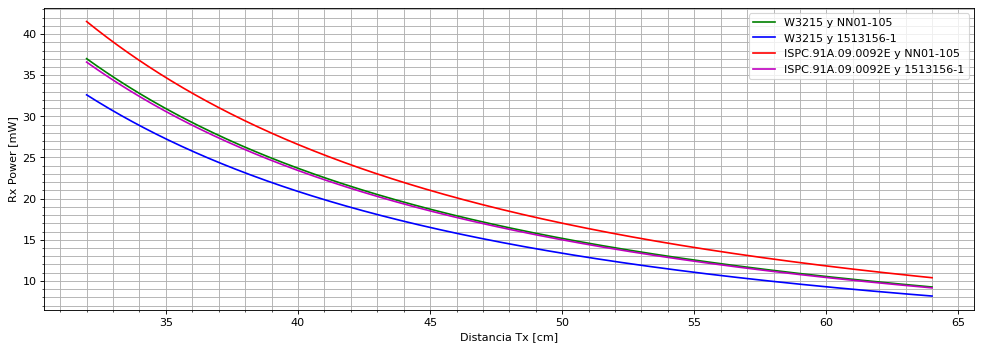
\includegraphics[width=\linewidth]{ImagenesFactibilidad/pot_recibida_teorica}
	\label{fig:pot_recibida_teorica}
	\caption{Potencia recibida en la antena Rx en función de la distancia entre antena Tx y antena Rx.}
\end{figure}

Se puede observar que con $4 \ W$ en la antena transmisora, todas las combinaciones de antenas cumplen con la potencia necesaria para el mejor y peor caso. Tomando el mejor par Rx-Tx, y al tener en cuenta la eficiencia de aproximadamente $70\%$ del P1110, la potencia a la salida de este permanece por encima del peor caso hasta la máxima distancia de transmisión.

\begin{figure}[H]
	\centering
	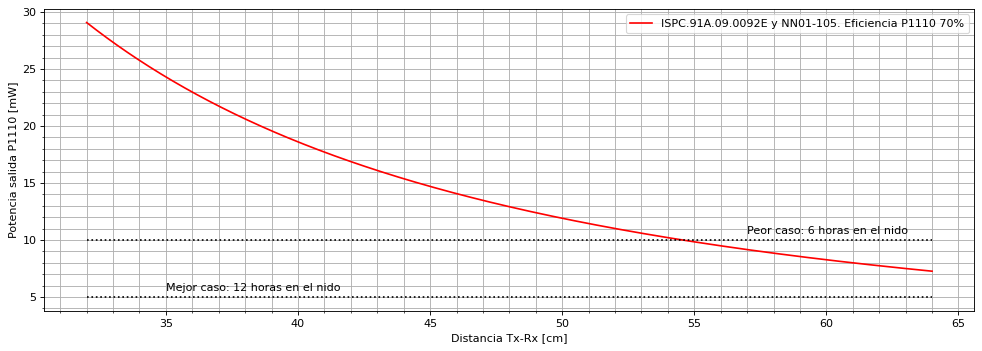
\includegraphics[width=\linewidth]{ImagenesFactibilidad/pot_baterias_teorica}
	\label{fig:pot_baterias_teorica}
	\caption{Potencia a la salida del P1110 en función de la distancia entre antena Tx y antena Rx.}
\end{figure}

Sin embargo, si se toma en consideración la restricción más estricta de $4.5 \  \frac{W}{m^2}$ impuesta en la Sección (\ref{sec:legal}) dada por la fórmula

\begin{equation}
	p = \frac{P_TG_T}{4\pi R^2}
\end{equation}

se observa en la Figura (\ref{fig:densidadradiada}) que para una potencia de $1.6 \ W$ en la antena transmisora esta restricción se cumple a treinta centímetros de la distancia mínima de transmisión.

\observacion{\verObs}{actualizar foto}
\begin{figure}[H]
	\centering
	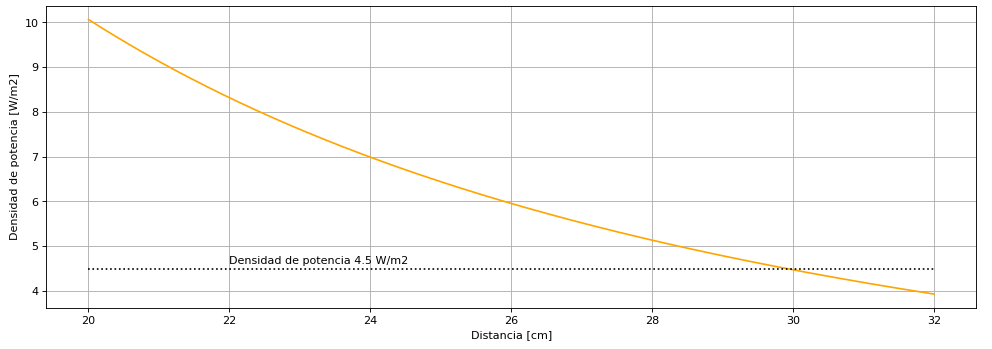
\includegraphics[width=\linewidth]{ImagenesFactibilidad/densidadradiada}
	\caption{Densidad de potencia radiada con $1.6 \ W$ en la antena transmisora según la fórmula de Friis.}
	\label{fig:densidadradiada}
\end{figure}

Teniendo esto en cuenta, y recalculando para $1.6 \ W$ se obtiene

\begin{figure}[H]
	\centering
	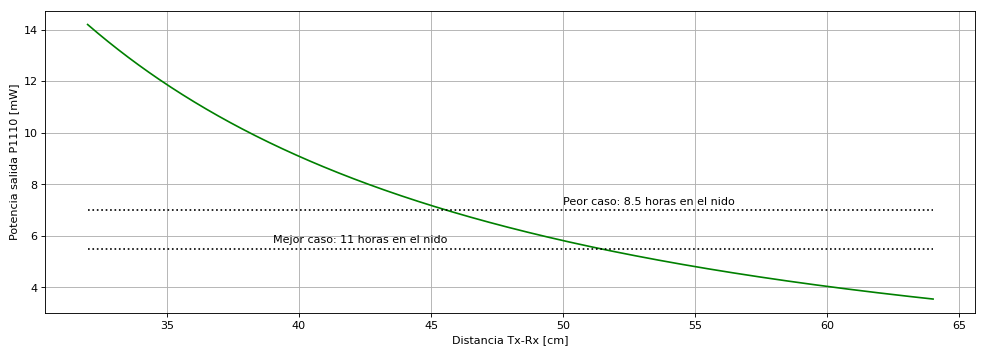
\includegraphics[width=\linewidth]{ImagenesFactibilidad/recalculo}
	\caption{Potencia a la salida del P1110 en función de la distancia entre antena Tx y antena Rx para $1.6 \ W$ en la antena transmisora.}
	\label{fig:recalculo}
\end{figure}

Por estas razones, se deberá complementar la recarga de la UBM utilizando un panel solar.
